% Options for packages loaded elsewhere
\PassOptionsToPackage{unicode}{hyperref}
\PassOptionsToPackage{hyphens}{url}
%
\documentclass[
]{article}
\usepackage{lmodern}
\usepackage{amssymb,amsmath}
\usepackage{ifxetex,ifluatex}
\ifnum 0\ifxetex 1\fi\ifluatex 1\fi=0 % if pdftex
  \usepackage[T1]{fontenc}
  \usepackage[utf8]{inputenc}
  \usepackage{textcomp} % provide euro and other symbols
\else % if luatex or xetex
  \usepackage{unicode-math}
  \defaultfontfeatures{Scale=MatchLowercase}
  \defaultfontfeatures[\rmfamily]{Ligatures=TeX,Scale=1}
\fi
% Use upquote if available, for straight quotes in verbatim environments
\IfFileExists{upquote.sty}{\usepackage{upquote}}{}
\IfFileExists{microtype.sty}{% use microtype if available
  \usepackage[]{microtype}
  \UseMicrotypeSet[protrusion]{basicmath} % disable protrusion for tt fonts
}{}
\makeatletter
\@ifundefined{KOMAClassName}{% if non-KOMA class
  \IfFileExists{parskip.sty}{%
    \usepackage{parskip}
  }{% else
    \setlength{\parindent}{0pt}
    \setlength{\parskip}{6pt plus 2pt minus 1pt}}
}{% if KOMA class
  \KOMAoptions{parskip=half}}
\makeatother
\usepackage{xcolor}
\IfFileExists{xurl.sty}{\usepackage{xurl}}{} % add URL line breaks if available
\IfFileExists{bookmark.sty}{\usepackage{bookmark}}{\usepackage{hyperref}}
\hypersetup{
  hidelinks,
  pdfcreator={LaTeX via pandoc}}
\urlstyle{same} % disable monospaced font for URLs
\usepackage{graphicx,grffile}
\makeatletter
\def\maxwidth{\ifdim\Gin@nat@width>\linewidth\linewidth\else\Gin@nat@width\fi}
\def\maxheight{\ifdim\Gin@nat@height>\textheight\textheight\else\Gin@nat@height\fi}
\makeatother
% Scale images if necessary, so that they will not overflow the page
% margins by default, and it is still possible to overwrite the defaults
% using explicit options in \includegraphics[width, height, ...]{}
\setkeys{Gin}{width=\maxwidth,height=\maxheight,keepaspectratio}
% Set default figure placement to htbp
\makeatletter
\def\fps@figure{htbp}
\makeatother
\setlength{\emergencystretch}{3em} % prevent overfull lines
\providecommand{\tightlist}{%
  \setlength{\itemsep}{0pt}\setlength{\parskip}{0pt}}
%\setcounter{secnumdepth}{-\maxdimen} % remove section numbering

\date{}

\begin{document}
\begin{titlepage}
    \begin{center}
        \textbf{\large Gymnázium, Praha 6, Nad Alejí 1952}\\
        \vspace{0.2cm}
        \rule{\textwidth}{0.5pt}\\
        \vspace{5cm}
        \textbf{\Huge Computatis}\\
        \vspace{5cm}
        \textbf{\large MATURITNÍ PRÁCE}\\
        \vspace{2cm}
        \textbf{\large Jakub Jelínek}\\
        \textbf{Oktáva A}\\
        \vspace*{\fill}
        \textbf{\large 2018/2019}\\
    \end{center}
\end{titlepage}
\newpage
Prohlašuji, že jsem tuto maturitní práci vypracoval samostatně a že je uvedena veškerá použitá literatura a další zdroje.\newline
\begin{minipage}{0.7\textwidth}
    \vspace{1cm}
    V Praze dne 15.4.2019
\end{minipage}
\begin{minipage}{0.3\textwidth}
    \vspace{1cm}
    \begin{flushright}
        \vspace{11pt}
        \hrulefill
    \end{flushright}
\end{minipage}
\newpage
\tableofcontents
\newpage

\section{O aplikaci}
Computatis je webová aplikace, která umožňuje uživateli procvičovat si matematiku.
Obsahuje několik příkladů, které jsou děleny do kategorií podle jevu, na který se zaměřují.
Každá otázka má odpověď, která lze jednoduše zapsat, aby se také jednoduše dala zkontrolovat,
což aplikace také ovládá. Po potvrzení odeslání výsledku se uživatel dozví, zda je výsledek správný, či chybný.

Webová stránka detailněji popisující aplikaci: 
\href{https://kubajj.gitlab.io/aboutcomputatis}{kubajj.gitlab.io/aboutcomputatis}

\section{Instalace}
\begin{itemize}
\item Nejdříve nainstalujte Node.js package manager, neboli npm.
\item Jděte do repozitáře této aplikace. (\texttt{cd\ computatis})
\item Spusťte příkaz \texttt{npm\ install}.
\item Spusťte příkaz \texttt{npm\ run\ dev}.
\end{itemize}
Pokud aplikaci nechcete vyvýjet, ale jen testovat, použijte k tomu demo:
\href{https://kubajj.gitlab.io/computatis}{kubajj.gitlab.io/computatis}

\section{Vývoj}
Všechny důležité soubory jsou v adresáři src. Ten je rozdělen na adresář \href{https://gitlab.com/kubajj/computatis/tree/master/src/assets}{assets}, kde se nalézají obrázky ikon,
adresář \href{https://gitlab.com/kubajj/computatis/tree/master/src/Content}{Content}, kde se nalézají vnořené komponenty, a na několik samostaných souborů.
\begin{itemize}
  \item App.vue
  \begin{itemize}
    \item Tento soubor definuje hlavní komponenty, které tvoří stránku. Je importován do index.html.
  \end{itemize}
  \item main.js  
  \begin{itemize}
    \item Tento soubor popisuje chování App.vue.
  \end{itemize}
  \item AppFooter.vue
  \begin{itemize}
    \item Definuje zápatí stránky.
  \end{itemize}
  \item Navigation.vue
  \begin{itemize}
    \item Definuje vzhled horní lišty stránky.
  \end{itemize}
  \item Logo.vue
  \begin{itemize}
    \item Vytvoří z loga stránky odkaz na domovskou stránku. 
  \end{itemize}
  \item routes.js
  \begin{itemize}
    \item Definuje chování routeru.
  \end{itemize}
\end{itemize}
Adresář \href{https://gitlab.com/kubajj/computatis/tree/master/src/Content}{Content} se dělí na dva samostatné soubory, které upravují obsah stránky, a na adresář 
\href{https://gitlab.com/kubajj/computatis/tree/master/src/Content/PracContentFiles}{PracContentFiles}. V tomto adresáři se nachází soubor 
\href{https://gitlab.com/kubajj/computatis/blob/master/src/Content/PracContentFiles/UvodKProcvicovani.vue}{UvodKProcvicovani.vue} a adresáře samostatných příkladů,
které jsou tematicky rozděleny.\\ Pro přidání nového komponentu je nutné sledovat pokyny ke zveřejnění komponentu:
\href{https://kubajj.gitlab.io/aboutcomputatis/#/vyvojar/zverejnenikomponentu}{kubajj.gitlab.io/aboutcomputatis/\#/vyvojar/zverejnenikomponentu}

\section{Ovládání aplikace}
Toto je návod k použití aplikace Computatis na procvičování matematiky.\\
V aplikaci je několik okruhů, ve kterých si můžete zvolit příklad k
procvičování, který se vám bude náhodně generovat. Výběr okruhů se
provádí pomocí tlačítek, které rozbalují seznam možných příkladů.\\

\includegraphics{../../doc-images/dropdown.png}\\
Tato tlačítka se nacházejí v
levé části tohoto bílého boxu.\\
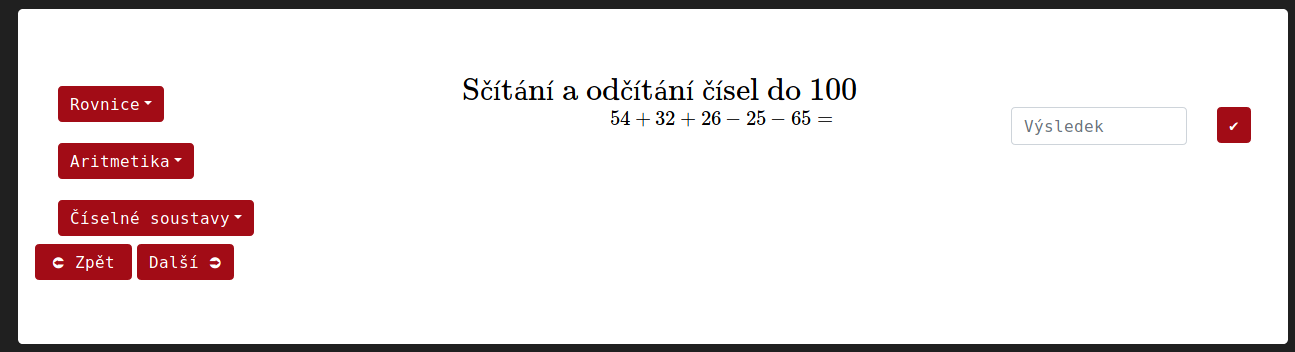
\includegraphics{../../doc-images/WhiteBox.png}\\
V pravé části se vám zobrazují zvolené příklady. Úplně vpravo můžete
zadat výsledek do formuláře.
\section{Příklady}
Příklady se generují náhodně, ale jejich výsledek je vždy jednoznačný.
Většinou je celočíselný (s výjimkou příkladu ``Lineární rovnice'', kde
je povolen i výsledek končící na .5 a .25) nebo slovní. Po potvrzení
výsledku buď klávesou ``Enter'', nebo tlačítkem vedle formuláře na
výsledek, se vám zobrazí zpráva, zda je váš výsledek správný a v
případě, že tomu tak není, se vám zobrazí i spravná odpověď.

Pokud si uživatel/ka není jist/a s postupem řešení, je možné kliknout na
tlačítko nápovědy. Nápovědy se od sebe liší. Některé zobrazí část
postupu, jiné zobrazí formulář, který má červený okraj. Tento okraj
zezelená, pokud je váš mezivýsledek správný (tento typ můžete najít
například v příkladu Násobení).

V dolní levé části bílého boxu se nacházejí tlačítka Zpět a Další.

\section{Nápovědy a funkce}

Tato část dokumentace popisuje nápovědy a funkce jednotlivých příkladů.

\subsection{Nápovědy v příkladu Kvadratická rovnice}

První nápověda vám ukáže rovnici uplavenou do obvyklého tvaru: ax2 + bx
+ c = 0.\\
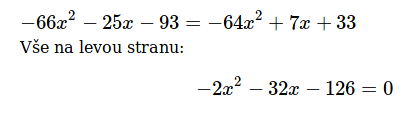
\includegraphics[width=6cm]{../../doc-images/zakladnitvar.png}\\
Další nápovědy se
liší v závislosti na tom, jak rovnice vyšla.\\
a) Diskriminant Tyto
nápovědy se zobrazí, pokud základní tvar rovnice má všechny 3 členy (a,
b, c).\\
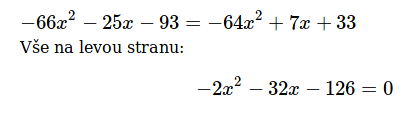
\includegraphics[width=6cm]{../../doc-images/zakladnitvar.png}\\
Následuje ukázání
vzorce pro diskriminant.\\
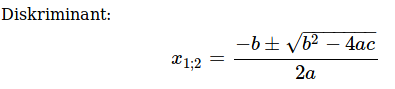
\includegraphics[width=6cm]{../../doc-images/diskriminant1.png}\\
Po stlačení tlačítka OK se zobrazí vzorec pro diskriminant s formuláři,
které kontrolují mezivýpočty.\\
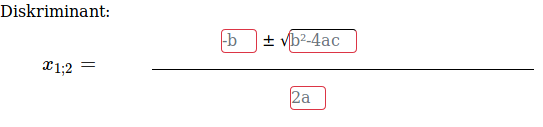
\includegraphics[width=8cm]{../../doc-images/diskriminant2.png}\\
Pokud jsou správně vyplněny, okraj jim zezelená.\\
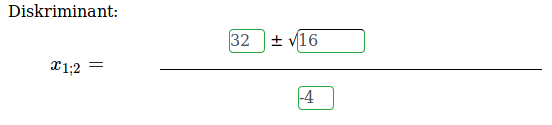
\includegraphics[width=8cm]{../../doc-images/diskriminant3.png}\\
Poté stačí jen upravit zlomek a zapsat výsledky.\\
b) Rozklad Tyto nápovědy se zobrazí, pokud
základní tvar rovnice nemá absolutní člen.\\
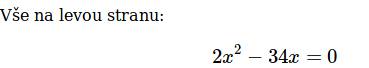
\includegraphics[width=6cm]{../../doc-images/rozklad1.png}\\
Tento typ nápovědy vytkne x
před závorku. Jeden výsledek bude tedy 0 a druhý vyjde, pokud je hodnota
závorky rovna 0.\\
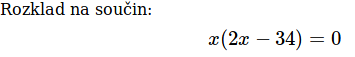
\includegraphics[width=6cm]{../../doc-images/rozklad2.png}\\
c) Odmocnění
Tyto nápovědy se zobrazí, pokud základní tvar rovnice nemá lineární
člen.\\
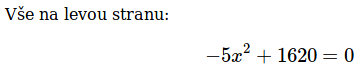
\includegraphics[width=6cm]{../../doc-images/odmocneni1.png}\\
Tento typ nápovědy
převede absolutní člen na druhou stranu rovnice. Výsledek vyjde po
odmocnění absolutního členu (výsledky budou 2 s opačným znaménkem).\\
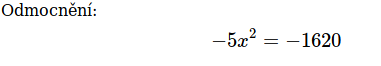
\includegraphics[width=6cm]{../../doc-images/odmocneni2.png}\\

\subsection{Sčítání a odčítání do 100}

Zobrazuje jednoduché výsledky na sčítání a odčítání do 100. Mezivýpočty
by také neměly vycházet větší než 100. Nápovědy u tohoto příkladu
vzhledem k jeho povaze nejsou implementovány.

\subsection{Násobení pod sebou}

Příklad na násobení trojciferného čísla dvojciferným. Po stlačení nápisu
``Chci násobit pod sebou'' se zobrazí formuláře s červeným okrajem. Po
zapsání odpovídajícího čísla okraj zezelená.\\
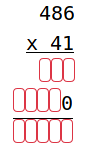
\includegraphics[height=2.5cm]{../../doc-images/multiblank.png}\\
Pokud uživatel vyplnil
poslední řádek formulářů správně, je to považováno za výsledek a může
postoupit k dalšímu příkladu.\\
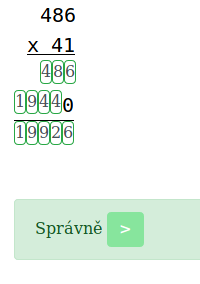
\includegraphics[height=4.5cm]{../../doc-images/multifull.png}\\

\subsection{Lineární rovnice}

Zobrazí linerání rovnici. Po stisknutí tlačítka nápovědy jsou všechny
lineární členy převedeny vlevo a absolutní vpravo. Uživatel už pouze
udělá podíl dvou čísel, která vycházejí buď jako celé číslo nebo zlomek
s číslem 2 nebo 4 ve jmenovateli.

\subsection{Adresy v paměti}

Tento příklad generuje náhodných 24 bajtů paměti. Uživatel je musí
analyzovat a splnit postupně 3 úkoly, které se vážou k jedné tabulce.\\
a) dvojkový doplněk\\
b) znaménkové rozšíření na daný počet bitů\\
c) určení endianity\\
Nápovědy u tohoto příkladu červeně zvýrazňují adresu/y, kterých se zadání týká.

\subsection{Převod mezi soustavami}

Příklad zadává jednoduché převody mezi soustavami (2;10;16). Uživatel
může stlačit tlačítko nápovědy, které nejdříve slovně popíše postup, jak
číslo převést.\\

\includegraphics{../../doc-images/slovni.png}\\
Po opětovném
kliknutí na tlačítko se ukáže formulář, který proces převodu rozdělí do
jednotlivých kroků s kontrolou mezivýsledků.\\

\includegraphics[width=6cm]{../../doc-images/formularova.png}\\

\newpage
\section{Zdroje}

\subsection{Použité knihovny}

\begin{itemize}
\tightlist
\item \LaTeX \url{https://www.latex-project.org/}
\item JavaScript \url{https://www.javascript.com}
\item Vue.js 2.5.22 \url{https://vuejs.org/}
\item Vue CLI 3.5.5 \url{https://cli.vuejs.org/}
\item Vue Router 3.0.2 \url{https://router.vuejs.org/}
\item BoostrapVue 2.0.0-rc.11 \url{https://bootstrap-vue.js.org/}
\item Vue Mathjax 0.0.6 \url{https://github.com/justforuse/vue-mathjax}
\item Npm 6.9.0 \url{https://www.npmjs.com/}
\item Webpack-simple \url{https://github.com/vuejs-templates/webpack-simple}
\item Webpack 3.6.0 \url{https://webpack.js.org/}
\item Html-webpack-plugin \url{https://github.com/jantimon/html-webpack-plugin}
\end{itemize}

\subsection{Dokumentace}

\begin{itemize}
\tightlist
\item Vuese/cli v2.3.0 \url{https://vuese.org/}
\item Pandoc \url{https://pandoc.org/}
\item Jakub Rada \url{https://github.com/JakubRada/Flashcards/}
\end{itemize}

\subsection{Ikony}

\begin{itemize}
\tightlist
\item IconFinder \url{https://www.iconfinder.com/icons/134216/hamburger_lines_menu_icon}
\item GNA \url{https://www.alej.cz/}
\end{itemize}

\subsection{Ostatní}

\begin{itemize}
\tightlist
\item W3Schools \url{https://www.w3schools.com/html/default.asp}
\item StackOverflow \url{https://stackoverflow.com/}
\item TheNetNinja \url{https://www.youtube.com/thenetninja}
\end{itemize}
\end{document}
